\section{Forundersøgelse}\label{ch:forundersoegelse}

\subsection{Medarbjeder-mål Tabel}
\begin{center}
\begin{longtable}{ |p{90pt}|p{90pt}|p{90pt}|p{90pt}| }
    \hline
    Medarbjeder & Opgave & Mål & Trin \\
    \hline\hline
    Ismand
    & Modtager ny ordre & Ordren er registreret som værende solgt. &
    - modtag ordre fra kunde \\
    &&&
    - Ordren med tilhørende adresse  registreres \\
    &&&
    - Adressen på ordren printes ud og lægges i den rigtige kasse til næste dag \\
    &&&
    - Den udprintede ordre tages med i bilen \\
    &&&
    - Ordren leveres til kunden på turen \\
    &&&
    - Kunden underskriver ordren \\
    &&&
    - Den underskrevene ordre afleveres til chefen \\
    \hline
    Ismand & Annuler ordre & Ordren er annulleret &
    - Modtag ordre fra kunde \\
    &&&
    - under “registrer ordre”, før samtlige trin er gennemført, kontakter kunden depotet og vil have ordre annulleret \\
    &&&
    - Ordren annulleres. \\
    \hline
    Lagermedarbejder
    & Isbilen skal ryddes op & Isbilens bokse er ryttet op så der er plads til nye varern &
    - Ismanden åbner en boks med is \\
    &&&
    - Ismanden omrokerer pakkerne således at der er bedre plads til nye pakker næste dag \\
    &&&
    - Ismanden lukker boksen \\
    &&&
    - Gentages indtil alle bokse er ryddet op. \\
    \hline
    Lagermedarbejder
    & Modtager nye varer & Varerne er registreret og lagt i fryseren &
    - Nye varer ankommer til depotet \\
    &&&
    - Varerne læsses af på paller \\
    &&&
    - Varerne registreres og godkendes så mængden stemmer \\
    &&&
    - Varerne lægges ind i fryseren \\
    \hline
    Lagermedarbejder & Varer skal afskrives & Varer er afskrevet &
    - Lageret er blevet talt op \\
    &&&
    - Under optælling er der fundet varer som er udløbet \\
    &&&
    - Varerne tilsidesættes \\
    &&&
    - Varerne registreres som udløbet i systemet \\
    &&&
    - Varerne er afskrevet og kan ikke sælges \\
    \hline
    Ismand & Isbilen skal ryddes op & Isbilens bokse er ryttet op så der er plads til nye varer & 
    - Ismanden åbner en boks med is \\
    &&&
    - Ismanden omrokerer pakkerne således at der er bedre plads til nye pakker næste dag \\
    &&&
    - Ismanden lukker boksen \\
    &&&
    - Gentages indtil alle bokse er ryddet op. \\
    \hline
    Lagermedarbejder & Isbilen skal påfyldes med is & Isbilen er påfyldt & 
    - Lagermedarbejder modtager bestillingsseddel, hvorpå der står hvor meget der skal fyldes på de forskellige biler. \\
    &&&
    - Lagermedarbejder fylder isene på en vogn inde i fryseren. Kører herefter vognen ud til isbilen og fylder på. \\
    \hline
    Bogfører (chef) & Mindstemængderne af isene skal opdateres & Mindstemængderne af isene er opdateret &
    - først undersøges hvilke is der har solgt godt og mindre godt \\
    &&&
    - Der laves en evaluering ud fra antallet solgt og nuværende mindstemængde på hver is \\
    &&&
    - Efter en manuel vurdering opdateres mindstemængderne så det passer til efterspørgslen. \\
    \hline
    Bogfører (chef) & Is skal bestilles hjem ud fra hvor mange is der mindst skal være på lager, og hvor mange is der skal være i hver bil & Is er bestilt hjem, i henhold til den manuelle vurdering af hvor mange der skal være. &
    - Undersøg hvor mange af hver is der blev solgt dagen før \\
    &&&
    - Lav en manuel vurdering af om mindste mængderne er i orden \\
    &&&
    - Lav en manuel vurdering af om nuværende antal på lageret er i orden \\
    &&&
    - Foretag ændringer af mindste mængder \\
    &&&
    - Bestil nye is hjem ud fra vurderingen så der er nok til næste gang \\
    \hline
    Ismand & Modtag nyt salg på ruten & Salget er registreret & 
    - På ruten kommer en kunde forbi bilen og vil købe is \\
    &&&
    - ismanden finder de ønskede varer \\
    &&&
    - varerne tilføjes til salget \\
    &&&
    - kundeoplysninger tilføjes til salget \\
    &&&
    - salget afsluttes \\
    &&&
    - Ordrebekræftelse til kunde, lager og regnskab \\
    \hline
    Chef & Medarbejderen skal evalueres hver måned &Medarbejderen er evalueret &
    - Medarbejderens præstationer ud fra målene læses \\
    &&&
    - Der laves en vurdering af hvilke områder medarbejderen skal fokusere på at gøre bedre \\
    &&&
    - Medarbejderen indkaldes til en samtale \\
    &&&
    - Medarbejderen for at vide hvilke områder der skal forbedres \\
    \hline
    Bogfører (chef) & Alle salg for dagen er afsluttet & Alle salgstal er bogført & 
    - Find all tallene for dagen \\
    &&&
    - åben et excel dokument til bogføring \\
    &&&
    - manuelt skriv af til excel dokumentet \\
    &&&
    - gem dokumentet. \\
    \hline
\end{longtable}
\end{center}

\subsection{Use Cases}
\textbf{Register ordre:} \\
En order modtages, på hjemmesiden. Alt afhængigt af hvor ordren registrets, vil den blive sendt ud til det nærmeste depot. f.eks hvis ordren er fra Nordjylland bliver det depotet i Aalborg, som har ansvaret for at ordren skal leveres. Herfra modtager chefen ordren og registere den, efterfuldt af dette, vil en printet seddel gives til en sælger, som registere ordren, når den bliver afleveret til kunden. 

\textbf{Annuller ordre:} \\
En kunde fortryder sin ordre, herfra kan kunden annulere orderen

\textbf{Afskriv vare:} \\
En lagermedarbejder finder en udgået varer og belyser depotchefen, som afskriver det i systemet. Herfra kan lagermedarbejderen smide varen ud. 

\textbf{Optælling af isbilen:} \\
Depot chefen tæller isbilen op, notere det ned og opdatere lager. 

\textbf{Modtag varer:} \\
En lagermedarbejder modtager varerne, når en lastbilerne fylder fryseren ud. Herfra registerer depotchefen de modtagede varer. 

\textbf{Bestil varer:} \\
Depotchefen holder øje med depotets fryser og fylder ud, når der er mangel på bestemt varer. Udover dette bestiller depotchefen flere af en bestemt varer hjem, når der er tilbud på en bestemt varer. 

\textbf{Kør salgsrute:} \\
En sælger modtager den bestemte rute, som sælgeren skal køre. Herfra indtaster sælgeren ruten ind i rutesystemet. Systemet finder ruten og nu er sælgeren klar til at køre ud med is. 

\textbf{Bogføring:} \\
Depotchefen tæller varene op, optæller om salgstallet stemmer overens. Herfra tastes tallene ind i excel. 

\textbf{Print ordrersedler:} \\
Depotchefen finder ordren og printer den ud. Herfra lægges den udprintede ordre på en hylde, som passer bedst med en af de kommende ruter.

\subsection{Use Case Diagram}

\begin{figure}[H]
    \centering
    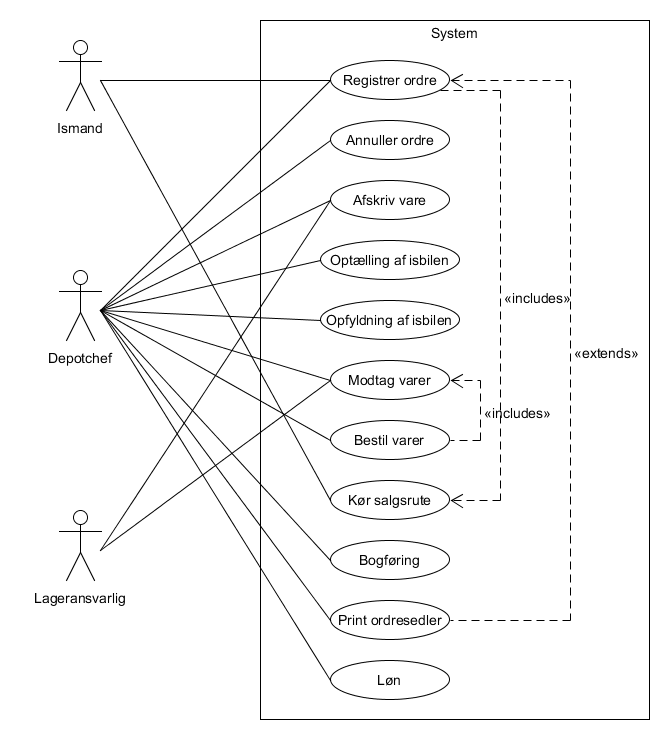
\includegraphics[width=\textwidth]{figures/Forundersøgelse/use_case_diagram.png}
    \caption{Use case diagram}
    \label{fig:use_case_diagram}
\end{figure}

\subsection{Workflow Diagrams}

\begin{figure}[H]
    \centering
    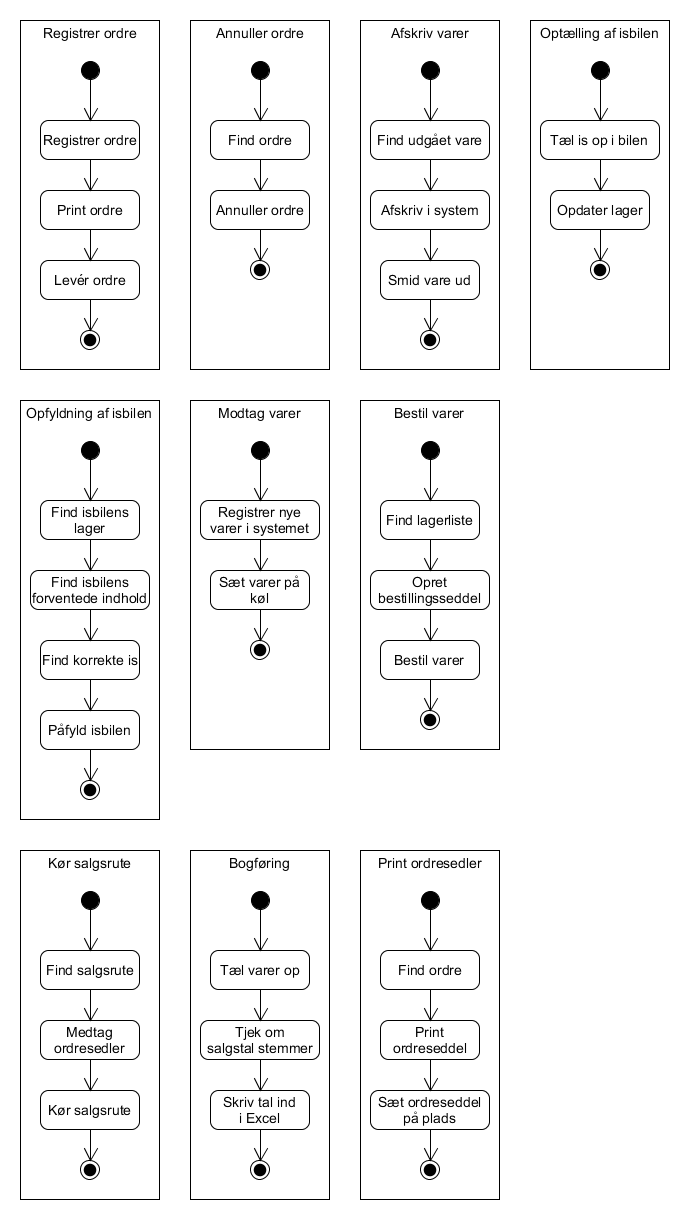
\includegraphics[width=0.9\textwidth]{figures/Forundersøgelse/workflows.png}
    \caption{Workflow diagram}
    \label{fig:workflows}
\end{figure}

\subsection{Brief Use Cases}\label{brief}
\textbf{Register ordre:}
En order modtages, på hjemmesiden. Alt afhængigt af hvor ordren registrets, vil den blive sendt ud til det nærmeste depot. f.eks hvis ordren er fra Nordjylland bliver det depotet i Aalborg, som har ansvaret for at ordren skal leveres. Herfra modtager chefen ordren og registere den, efterfuldt af dette, vil en printet seddel gives til en sælger, som registere ordren, når den bliver afleveret til kunden. 

\textbf{Annuller ordre:}
En kunde fortryder sin ordre, herfra kan kunden annulere orderen

\textbf{Afskriv vare:} 
En lagermedarbejder finder en udgået varer og belyser depotchefen, som afskriver det i systemet. Herfra kan lagermedarbejderen smide varen ud. 

\textbf{Optælling af isbilen:} 
Depot chefen tæller isbilen op, notere det ned og opdatere lager. 

\textbf{Modtag varer:} 
En lagermedarbejder modtager varerne, når en lastbilerne fylder fryseren ud. Herfra registerer depotchefen de modtagede varer. 

\textbf{Bestil varer:} 
Depotchefen holder øje med depotets fryser og fylder ud, når der er mangel på bestemt varer. Udover dette bestiller depotchefen flere af en bestemt varer hjem, når der er tilbud på en bestemt varer. 

\textbf{Kør salgsrute:} 
En sælger modtager den bestemte rute, som sælgeren skal køre. Herfra indtaster sælgeren ruten ind i rutesystemet. Systemet finder ruten og nu er sælgeren klar til at køre ud med is. 

\textbf{Bogføring:}
Depotchefen tæller varene op, optæller om salgstallet stemmer overens. Herfra tastes tallene ind i excel. 

\textbf{Print ordrersedler:}
Depotchefen finder ordren og printer den ud. Herfra lægges den udprintede ordre på en hylde, som passer bedst med en af de kommende ruter.

\subsection{Mock ups og designprincipper}
Når det kommer til at designe en brugergrænseflade til sit system, er der indtil flere overvejelser man skal igennem. Målet er at gøre brugergrænsefladen så brugervenlig, hurtig og intuitiv som mulig. Dette afsnit vil derfor gennemgå hvilke overvejelser der er indgået i beslutningen for designet af de anvendte mock ups.

\subsubsection{Farver}
Farver i et professionelt UI system kan være en definerende faktor. Farven må ikke være for meget til stede, men giver blot en identitet til programmet. I programmer som Spotify og Visual Studio Code har de begge en identitetsfarve, henholdsvis grøn og blå, men farven ses kun vigtige steder i programmet. 
\begin{figure}
    \centering
    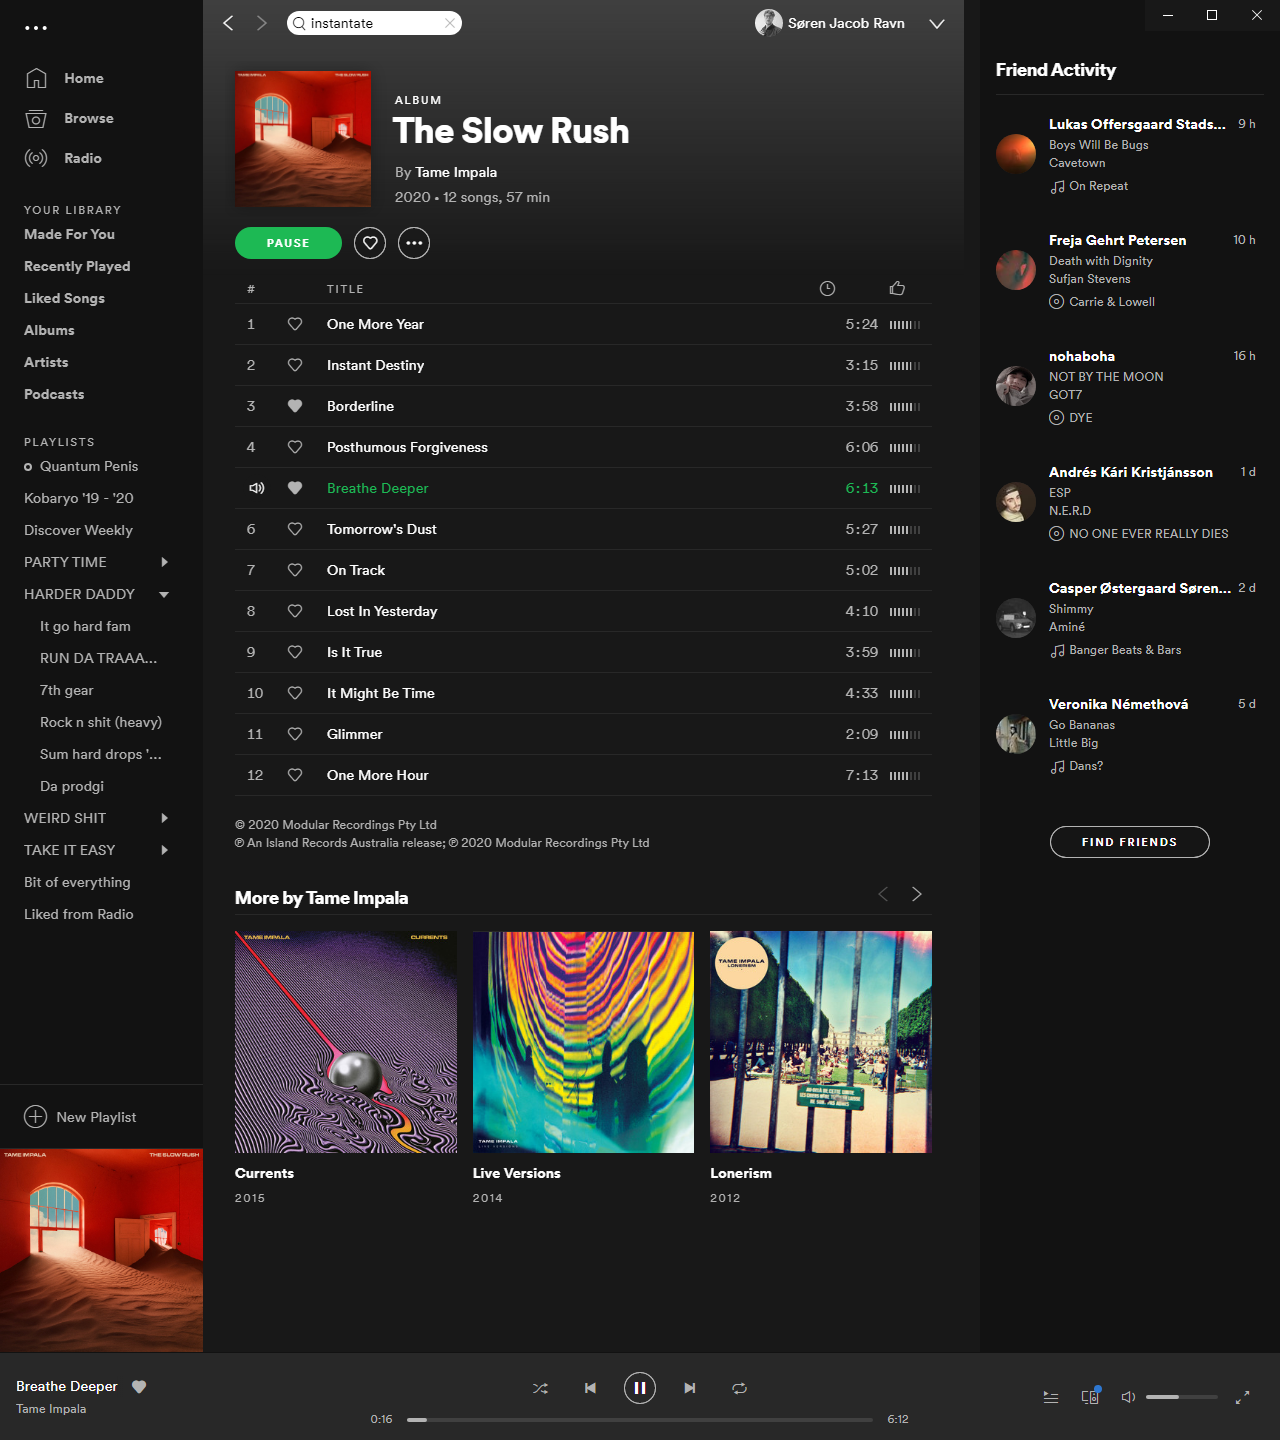
\includegraphics[width=\textwidth]{figures/Preliminary/Spotify.png}
    \label{fig:spotify}
\end{figure}
Som det kan ses forekommer den grønne farve i Spotify kun på den store Play/Pause knap, den sang man er i gang med, og hvilken enhed man bruger sin konto fra. Den grønne farve fylder knap 2\% af programmets brugergrænseflade, og fungerer godt sammen med de meget mørke og grå farver. 
På Hjem-IS' hjemmeside \cite{hjemis} er der allerede en god farvepalet, med både mørke og lyse farver. 
\begin{figure}
    \centering
    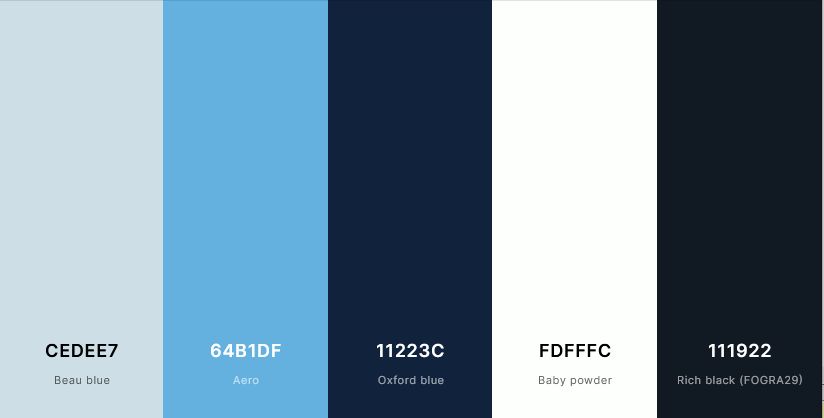
\includegraphics[width=\textwidth]{figures/Preliminary/farvepalet.png}
    \label{fig:farvepalet}
\end{figure}
Da blå er fokusfarven for Hjem-IS, er det vigtigt også at forstå betydningen af den farve. Den blå farve kan betyde tillid, rolighed, fred, og loyalitet. Disse ord passer godt med beskrivelsen af Hjem-IS' forhold med Danmark og dets kultur fra organisationsundersøgelsen. Til selve brugergrænsefladen, tages der en beslutning om at den mest brugte farve til baggrunden vil være Baby powder (FDFFFC). Hertil vil mindre kasser eller områder være i Oxford blue (11223C) og så vil der bruges Aero (64B1DF) til få highlights. Disse farver giver kontrast så det er nemt at se hvad der er i fokus, men samtidig komplimenterer farverne hinanden. Udover paletten vil der også blive benyttet mild grøn og mild rød til tal for at symbolisere, hvordan de ligger i forhold til budget.

\subsubsection{Skrifttype}
Skrifttypen Segoe UI Black er valgt fordi den minder meget om skrifttypen anvendt på Hjem-IS' hjemmeside \cite{hjemis}. Skrifttypen er tyk, rund og ikke så skarp. Disse ord kan også beskrive deres produkter, hvilket giver god sammenhæng.
penis musik er godt :)


